\chapter{Thực nghiệm và kết quả}
\label{chap:ket-qua}

Mọi con số trong chương là phần trăm (Acc@$k$) hoặc điểm phần trăm ($\Delta$), sinh tự động từ dữ liệu; khoảng trong
ngoặc vuông là khoảng tin cậy \ConstCiLevel\% bootstrap theo cụm khuôn mẫu, không hiệu chỉnh đa so sánh. Trừ khi ghi
khác, kết quả là của Gemini 3.8 Flash, ba lần chạy, trên tập test.

\section{RQ1 -- Tái hiện và kiểm tra cách đánh giá}
\label{sec:rq1}

\textbf{Tái hiện và cách chấm.} Tính lại từ nhật ký công bố khớp cả 13 cấu hình của SemLoc; \emph{chạy lại} với Claude
Sonnet 4.6 trên tập dev thì không (Acc@1 \RepClaudeDevRerunAccOne\% so với \RepClaudeDevPublishedAccOne\%, Acc@3
\RepClaudeDevRerunAccThree\% so với \RepClaudeDevPublishedAccThree\%). Mã chấm điểm công bố cho gỡ lỗi chia đôi \RqOneDdAuthorAllAccOne\% (bài báo ghi 0, chấm công bằng
cho \RqOneDdFairAllAccOne\%) và đánh giá thấp SBFL (Ochiai) ở top-5 (\RqOneSbflOchiaiAuthorAllAccFive\% so với
\RqOneSbflOchiaiFairAllAccFive\% khi dùng hạng trung bình). SemLoc gần như không đổi khi chấm công bằng, nhưng bỏ
\emph{điểm thưởng cho dòng LLM tự đoán} (thành phần không có trong bài báo) làm Acc@1 đi từ
\RqOneSemlocClaudeTZeroEightFairAllAccOne\% xuống \RqOneSemlocClaudeTZeroEightNoPriorFairAllAccOne\% (Claude) và từ
\RqOneSemlocGeminiTZeroEightFairAllAccOne\% xuống \RqOneSemlocGeminiTZeroEightNoPriorFairAllAccOne\% (Gemini).

\textbf{Kiểm chứng phản thực tế và lỗi gói mã.} Kết quả vá thử được tính nhưng \emph{không dùng để xếp hạng}: thứ hạng có
và không có bước này trùng nhau ở cả 250 chương trình, dù nó chiếm \CostCfSharePct\% lượt gọi LLM của SemLoc. Bộ chạy
BugsInPy công bố báo hạng của chính dòng LLM đoán và để lại \texttt{.pyc} của bản đã vá; nhóm đã khắc phục cả hai.

\textbf{Chất lượng nhãn.} Hình~\ref{fig:nhan-goc} cho thấy trên \LabaudAllN{} chương trình chỉ \LabaudAllSame{} nhãn
giữ nguyên, \LabaudAllExtended{} nhãn được thêm một dòng và \LabaudAllMoved{} nhãn bị dời (dòng trống \LabaudAllBlank,
dòng không phải mã \LabaudAllNonCode, lệch một dòng \LabaudAllOffByOne, xa hơn \LabaudAllFarther). Duyệt mù ủng hộ các
lần dời: trong \BlindBlindAllNReviewed{} câu trả lời mù, \BlindBlindAllMatchReviewed{} trùng nhãn đã rà soát và chỉ
\BlindBlindAllMatchOriginal{} trùng nhãn gốc. Chỗ khó nhất là lỗi thiếu câu lệnh (\BlindBlindKeptMatchReviewed{}/\BlindBlindKeptNReviewed{} ở nhóm nhãn giữ
nguyên), nơi nhãn cấp dòng vốn mơ hồ.

\begin{figure}[H]
\centering
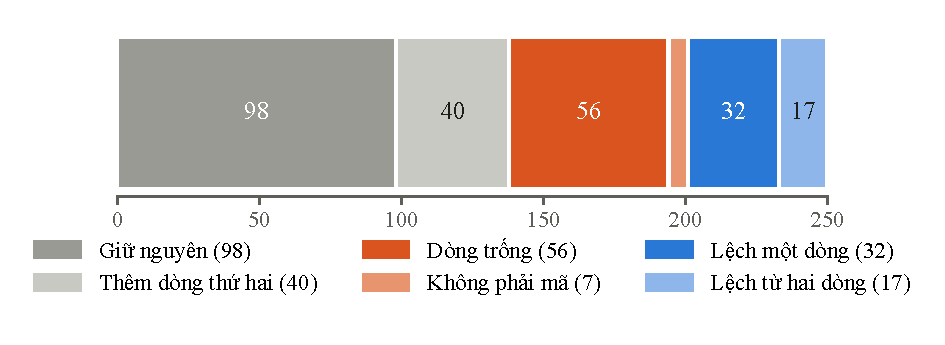
\includegraphics{../generated/vi/fig_label_flow.pdf}
\caption{Nhãn gốc của 250 chương trình so với nhãn đã rà soát: giữ nguyên, thêm dòng thứ hai (lỗi trải hai dòng), hoặc bị dời (dòng trống, dòng không phải mã, lệch một dòng, lệch từ hai dòng trở lên)}
\label{fig:nhan-goc}
\end{figure}

Nhãn lệch có thể đã có lợi cho SemLoc, vốn xếp nhiều dòng liền nhau: hơn LLM-Direct ở Acc@3 trên nhãn gốc
(\RqTwoOriginalAllSemlocAccThreeMean\% so với \RqTwoOriginalAllLlmDirectAccThreeMean\%) nhưng ngang trên nhãn đã rà soát
($\Delta$ \RqTwoReviewedAllLlmDirectDAccThree{} [\RqTwoReviewedAllLlmDirectDAccThreeLo; \RqTwoReviewedAllLlmDirectDAccThreeHi]).

\label{sec:overclaim}%
Bài báo SemLoc có những chỗ \emph{tuyên bố quá mức} (overclaim): khẳng định mạnh hơn mức bằng chứng của chính nó cho phép.
Bản thân điểm thưởng cho dòng LLM đoán là một lựa chọn thiết kế; chỗ tuyên bố quá mức là bài báo quy độ chính xác cho bằng
chứng thực thi trong khi không mô tả điểm thưởng quyết định hạng 1. Bảng~\ref{tab:overclaim} đặt từng khẳng định cạnh điều nhóm kiểm tra được.

\begin{table}[H]
\centering
\caption{Khẳng định của bài báo SemLoc và kết quả kiểm tra của nhóm}
\label{tab:overclaim}
{\setstretch{1.15}\small
\begin{tabularx}{\linewidth}{@{}>{\raggedright\arraybackslash}p{0.36\linewidth}>{\raggedright\arraybackslash}X@{}}
\toprule
Bài báo khẳng định & Nhóm kiểm tra thấy \\
\midrule
Độ chính xác đến từ việc neo lập luận của LLM vào bằng chứng thực thi &
  Dòng LLM tự đoán luôn đứng hạng 1 nhờ điểm thưởng \ConstPriorWeight{} không được mô tả trong bài báo; bỏ điểm thưởng,
  Acc@1 (nhãn đã chuẩn hóa) đi từ \RqTwoRepairedAllSemlocAccOneMean\% xuống \RqTwoRepairedAllSemlocNoPriorAccOneMean\% \\
Bước kiểm chứng phản thực tế (vá thử) xác nhận dòng lỗi &
  Kết quả vá thử không được dùng để xếp hạng: thứ hạng trùng nhau ở cả 250 chương trình, dù bước này chiếm
  \CostCfSharePct\% lượt gọi LLM \\
Acc@1 \RqOneSemlocClaudeTZeroEightAuthorAllAccOne\% trên SemFault-250 &
  Được chấm trên bộ nhãn có \GtBlankN{} nhãn nằm trên dòng trống và \GtNotExecutedN{} chương trình không kiểm thử thất bại
  nào chạy tới nhãn \\
Kết quả báo cáo từ một lần chạy &
  Không có khoảng tin cậy hay kiểm định; nhóm lặp mỗi cấu hình ba lần và báo khoảng tin cậy \ConstCiLevel\% bootstrap \\
\bottomrule
\end{tabularx}}
\end{table}

\section{RQ2 -- Một prompt có kiểm thử thất bại so với quy trình nhiều bước}
\label{sec:rq2}
\label{sec:failloc-vs-semloc}

\textbf{FailLoc} thắng SemLoc ở Acc@1 trên cả ba bộ nhãn (Bảng~\ref{tab:ket-qua-chinh}, Hình~\ref{fig:ket-qua-chinh}):
\RqTwoOriginalAllLlmTestsDAccOne{} [\RqTwoOriginalAllLlmTestsDAccOneLo; \RqTwoOriginalAllLlmTestsDAccOneHi] trên bộ gốc,
\RqTwoRepairedAllLlmTestsDAccOne{} [\RqTwoRepairedAllLlmTestsDAccOneLo; \RqTwoRepairedAllLlmTestsDAccOneHi] trên bộ đã
chuẩn hóa và \RqTwoReviewedAllLlmTestsDAccOne{} [\RqTwoReviewedAllLlmTestsDAccOneLo; \RqTwoReviewedAllLlmTestsDAccOneHi]
trên bộ đã rà soát. Ở Acc@3 nó hơn \RqTwoRepairedAllLlmTestsDAccThree{} [\RqTwoRepairedAllLlmTestsDAccThreeLo;
\RqTwoRepairedAllLlmTestsDAccThreeHi] trên bộ đã chuẩn hóa; trên nhãn gốc khoảng tin cậy chứa 0 vì có lỗi không kiểm thử
nào chạy tới (chỉ tính lỗi được chạy tới: \RqTwoOriginalExecutableLlmTestsDAccThree{}
[\RqTwoOriginalExecutableLlmTestsDAccThreeLo; \RqTwoOriginalExecutableLlmTestsDAccThreeHi]). FailLoc tốn
\CostLlmTestsTokensK{} nghìn token mỗi chương trình so với \CostSemlocTokensK{} nghìn của SemLoc (Hình~\ref{fig:chi-phi});
SBFL (Ochiai) thấp nhất ở Acc@1 và Acc@3 trên mọi bộ nhãn. Ở Acc@5, FailLoc đạt \RqTwoRepairedAllLlmTestsAccFiveMean\% so với
\RqTwoRepairedAllSemlocAccFiveMean\% của SemLoc trên bộ đã chuẩn hóa, nhưng trên nhãn gốc SemLoc cao hơn
(\RqTwoOriginalAllSemlocAccFiveMean\% so với \RqTwoOriginalAllLlmTestsAccFiveMean\%); FailLoc chỉ trả về năm dòng. Trên một tập con
(\ParetoSemlocGeminiThreeEightFlashN{} chương trình), FailLoc+Cov có Acc@3 cao hơn và tốn ít token hơn SemLoc với cả năm mô
hình (Hình~\ref{fig:pareto}; chưa có khoảng tin cậy). Trên bộ đã rà soát FailLoc đạt Acc@3 \RqTwoReviewedAllLlmTestsAccThreeMean\%:
SemFault-250 gần như bão hòa với một prompt đơn giản (Mục~\ref{chap:that-bai}).

\begin{table}[H]
\centering
\caption{Kết quả chính trên ba bộ nhãn (tập test, Gemini 3.8 Flash, trung bình 3 lần chạy) và chi phí token mỗi chương trình}
\label{tab:ket-qua-chinh}
\resizebox{\linewidth}{!}{\begin{tabular}{lrrrrrrr}
\toprule
 & \multicolumn{2}{c}{Bản gốc ($n=200$)} & \multicolumn{2}{c}{Đã chuẩn hóa ($n=190$)} & \multicolumn{2}{c}{Đã rà soát ($n=200$)} & \\
\cmidrule(lr){2-3}\cmidrule(lr){4-5}\cmidrule(lr){6-7}
Phương pháp & Acc@1 & Acc@3 & Acc@1 & Acc@3 & Acc@1 & Acc@3 & nghìn token \\
\midrule
SBFL (Ochiai) & 3,0 & 15,5 & 3,7 & 18,4 & 11,0 & 28,0 & 0 \\
LLM-Direct & 40,0 & 43,0 & 58,8 & 64,9 & 87,3 & 90,8 & 2,5 \\
SemLoc & 36,8 & 60,3 & 53,9 & 76,0 & 83,0 & 90,0 & 14,0 \\
FailLoc (nhóm đề xuất) & 44,5 & 67,5 & 64,2 & 90,5 & 95,5 & 100,0 & 2,0 \\
FailLoc+Cov & 40,2 & 68,2 & 58,6 & 92,5 & 92,2 & 100,0 & 2,6 \\
\bottomrule
\end{tabular}
}
\end{table}

\begin{figure}[H]
\centering
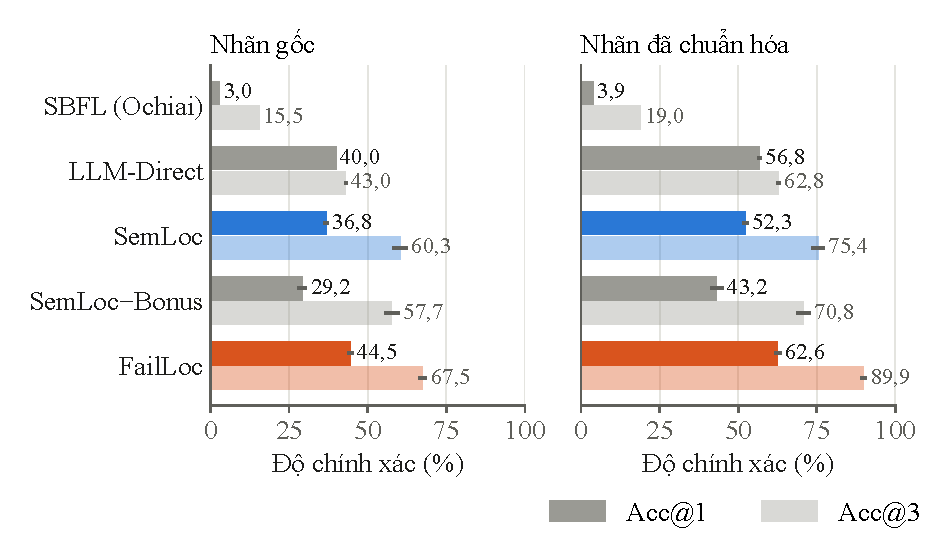
\includegraphics{../generated/vi/fig_rq2_main.pdf}
\caption{Kết quả chính trên tập test (Gemini 3.8 Flash): Acc@1 (cột đậm) và Acc@3 (cột nhạt) trên nhãn gốc và nhãn đã chuẩn hóa, trung bình ba lần chạy; vạch là độ lệch chuẩn giữa các lần chạy. FailLoc màu cam, SemLoc màu xanh}
\label{fig:ket-qua-chinh}
\end{figure}

\begin{figure}[H]
\centering
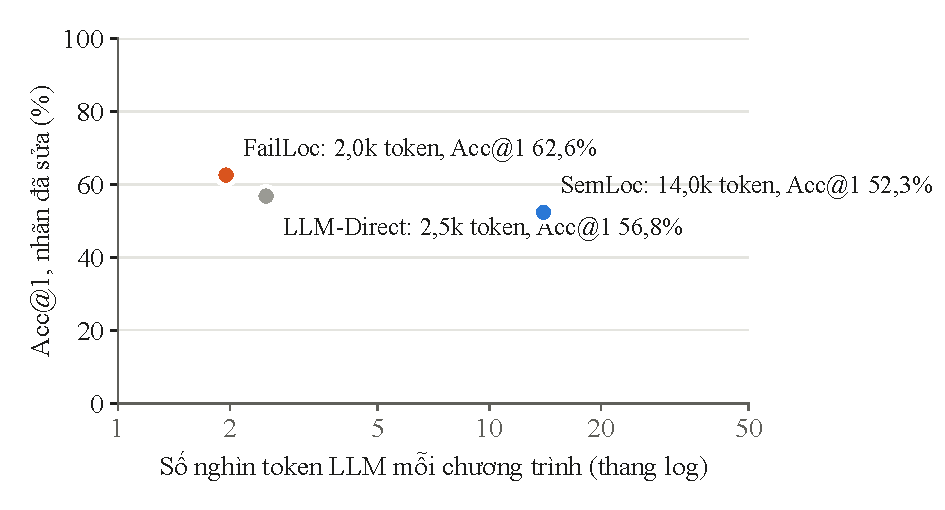
\includegraphics{../generated/vi/fig_cost_acc.pdf}
\caption{Chi phí và độ chính xác trên tập test với cùng mô hình: số token LLM trung bình mỗi chương trình (thang log) và Acc@1 trên nhãn đã chuẩn hóa}
\label{fig:chi-phi}
\end{figure}

\begin{figure}[H]
\centering
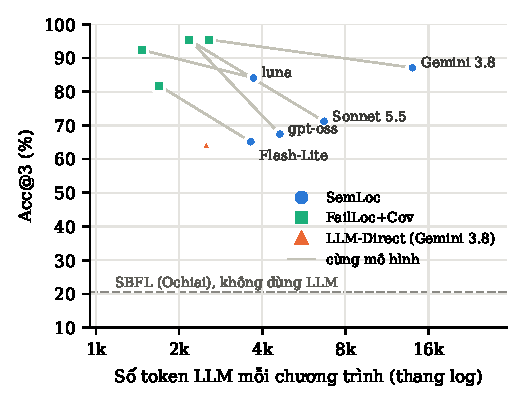
\includegraphics[width=0.75\linewidth]{../generated/vi/pareto.pdf}
\caption{Chi phí và độ chính xác (Acc@3) trên cùng tập con, nhãn đã chuẩn hóa; đường nối hai phương pháp của cùng một mô hình}
\label{fig:pareto}
\end{figure}

\label{sec:do-nhay-nhan}%
Phần lớn ca trượt chỉ vào dòng kề cạnh trong cặp điều kiện -- câu lệnh nó bảo vệ (Mục~\ref{sec:mo-ho}); chỉ số
phụ \emph{Acc@1 nới lỏng} (đặt ra sau khi thấy kết quả) chấp nhận cả dòng kia trong cặp. Trên bộ đã chuẩn hóa, nới lỏng đưa SemLoc từ \RqtolRepairedSemlocAccOneExact\% lên
\RqtolRepairedSemlocAccOneTol\% và FailLoc từ \RqtolRepairedLlmTestsAccOneExact\% lên \RqtolRepairedLlmTestsAccOneTol\%;
kết luận không đổi: FailLoc vẫn hơn SemLoc \RqtolRepairedLlmTestsDAccOneTol{} [\RqtolRepairedLlmTestsDAccOneTolLo;
\RqtolRepairedLlmTestsDAccOneTolHi] điểm.

\section{RQ3 -- FailLoc thắng nhờ đâu?}
\label{sec:rq3}

\subsection{Tín hiệu nào tạo ra khác biệt}

\textbf{Kiểm thử thất bại} là tín hiệu chính (Hình~\ref{fig:ablation}): so với LLM-Direct nó thay đổi Acc@3
\AblRepairedAllTestsEffectDAccThree{} [\AblRepairedAllTestsEffectDAccThreeLo; \AblRepairedAllTestsEffectDAccThreeHi]
điểm trên bộ đã chuẩn hóa. \textbf{Độ phủ từng dòng} không giúp: FailLoc+Cov thay đổi Acc@3
\AblRepairedAllCoverageEffectDAccThree{} [\AblRepairedAllCoverageEffectDAccThreeLo; \AblRepairedAllCoverageEffectDAccThreeHi]
và Acc@1 \AblRepairedAllCoverageEffectDAccOne{} [\AblRepairedAllCoverageEffectDAccOneLo;
\AblRepairedAllCoverageEffectDAccOneHi] trên bộ đã chuẩn hóa. Giả thuyết H3 bị bác bỏ: LLM cần biết \emph{kiểm thử nào
thất bại và vì sao}, không cần biết dòng nào được chạy qua.

\begin{figure}[H]
\centering
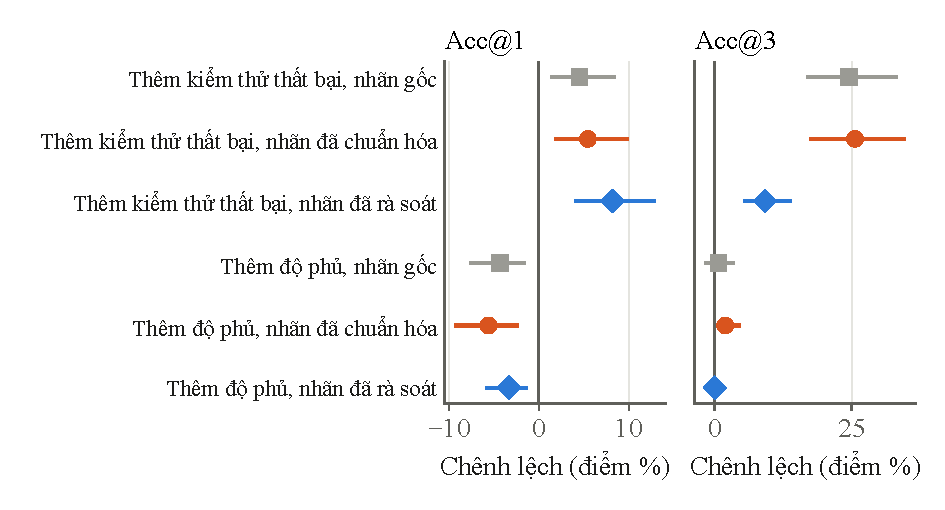
\includegraphics{../generated/vi/fig_ablation.pdf}
\caption{Ablation trên prompt (tập test, Gemini 3.8 Flash, ba lần chạy): chênh lệch khi thêm kiểm thử thất bại (LLM-Direct sang FailLoc) và khi thêm độ phủ từng dòng (FailLoc sang FailLoc+Cov), với khoảng tin cậy \ConstCiLevel\% bootstrap}
\label{fig:ablation}
\end{figure}

\label{sec:phan-ra}%
Ở phía SemLoc, phân rã Shapley tách tín hiệu dòng đoán khỏi phổ vi phạm để kiểm giả thuyết H1. Vì điểm thưởng lớn hơn mọi điểm ràng buộc, \textbf{hạng 1 của SemLoc là ``guessed'' theo thiết kế}
(Hình~\ref{fig:phan-ra}): riêng dòng đoán và SemLoc cùng đạt Acc@1 \RqTwoRepairedAllSemlocAccOneMean\% trên bộ đã chuẩn
hóa, riêng phổ đạt \RqTwoRepairedAllSemlocNoPriorAccOneMean\%. Ở top-3 phổ có tác dụng thật (riêng phổ
\RqTwoRepairedAllSemlocNoPriorAccThreeMean\%, cả hai \RqTwoRepairedAllSemlocAccThreeMean\%), nhưng FailLoc đạt top-3 cao
hơn mà không cần phổ. Riêng phổ đạt Acc@1 thấp hơn SemLoc, nên giả thuyết H1 không bị bác bỏ.

\begin{figure}[H]
\centering
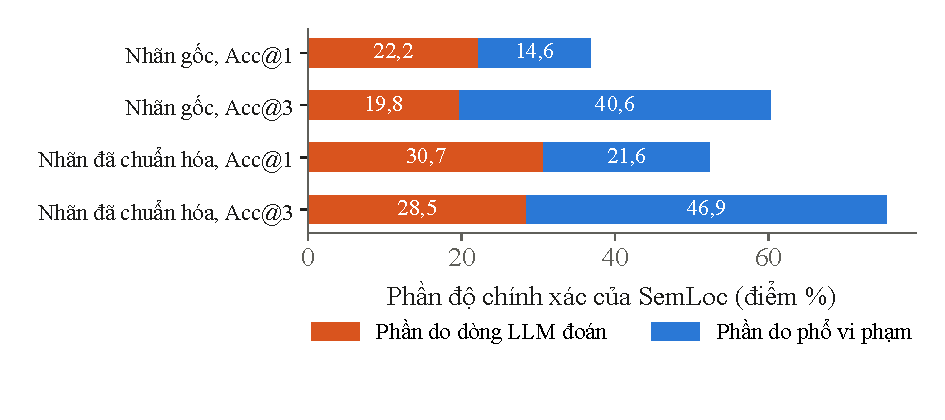
\includegraphics{../generated/vi/fig_decomposition.pdf}
\caption{Phân rã Shapley độ chính xác của SemLoc (tập test, ba lần chạy Gemini 3.8 Flash) thành phần do dòng LLM đoán và phần do phổ vi phạm}
\label{fig:phan-ra}
\end{figure}

\subsection{Các cách bổ sung không thu hẹp được khoảng cách với FailLoc}

Hình~\ref{fig:bo-sung} đặt các cách bổ sung cạnh nhau. CovGate (phá hòa bằng Ochiai) thay đổi Acc@3 của SemLoc
\RqTwoRepairedAllCovgateDAccThree{} [\RqTwoRepairedAllCovgateDAccThreeLo; \RqTwoRepairedAllCovgateDAccThreeHi] điểm và không
đổi Acc@1. FailLoc+Verify được báo qua hai cấu hình:
\emph{FailLoc+MinFix} kiểm hai dòng đầu và chỉ nhận bản sửa một token (cấu hình có Acc@1 cao nhất trên tập dev),
\emph{FailLoc+AnyFix} kiểm ba dòng đầu và nhận bản sửa bất kỳ (thấp nhất trên tập dev). Trên tập dev với nhãn đã rà
soát, FailLoc+MinFix đạt Acc@1 \PavDevChosenReviewedAccOne\% so với \PavDevStageReviewedAccOne\% của FailLoc, còn
FailLoc+AnyFix chỉ đạt \PavDevWorstReviewedAccOne\%: bản sửa nhỏ làm mọi kiểm thử đạt ở \PavmechReviewedFaultLineFixable\% lần kiểm tại
dòng lỗi thật nhưng cũng ở \PavmechReviewedOtherLineFixable\% lần tại dòng không lỗi, nên không phân biệt được (trên tập
test hai tỉ lệ này là \PavmechtestReviewedFaultLineFixable\% và \PavmechtestReviewedOtherLineFixable\%).
Chạy lại trên tập test (ba lần, tham số giữ nguyên như trên dev), FailLoc+MinFix không đổi dòng đứng đầu nào
nên Acc@1 và Acc@3 bằng đúng FailLoc (\PavtestChosenReviewedPavAccOne\% với nhãn đã rà soát); FailLoc+AnyFix đổi
dòng đứng đầu \PavtestWorstReviewedTopOneChanged{} lần và làm Acc@1 giảm \PavtestWorstReviewedDAccOne{}
[\PavtestWorstReviewedDAccOneLo; \PavtestWorstReviewedDAccOneHi] điểm.
FailLoc+Vote không cải thiện: trên tập dev nó làm Acc@3 đi xuống trên bộ đã chuẩn hóa (\VoteRepairedVoteAccThree\% so với
\VoteRepairedSingleAccThree\%); trên tập test, gộp ba lần chạy FailLoc chỉ đổi Acc@1 \VotetestRepairedDAccOne{}
[\VotetestRepairedDAccOneLo; \VotetestRepairedDAccOneHi] điểm, khoảng tin cậy chứa 0. Phân tích tĩnh
gần như không chỉ ra dòng lỗi: Ruff (mọi luật) trúng \StatReviewedRuffAllOnFaultLine{} chương trình, Pyrefly không lần nào.

\begin{figure}[H]
\centering
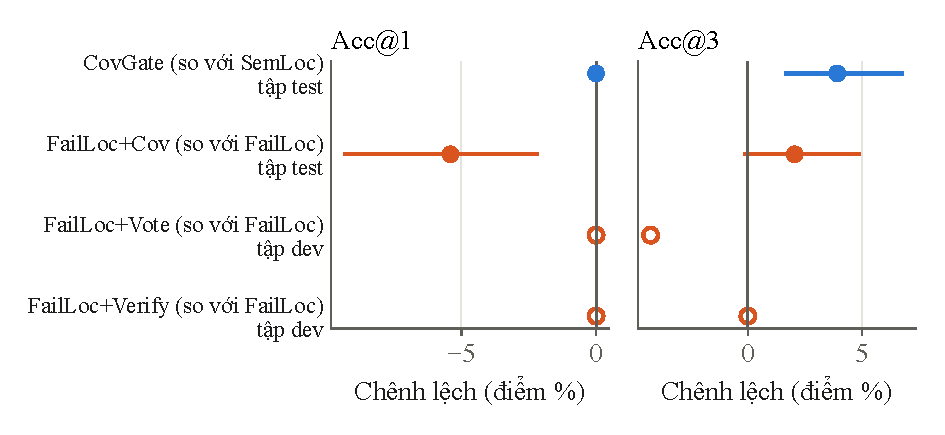
\includegraphics{../generated/vi/fig_addons.pdf}
\caption{Chênh lệch của từng cách bổ sung so với phương pháp nó mở rộng (nhãn đã chuẩn hóa). Điểm đặc có khoảng tin cậy \ConstCiLevel\% (tập test, ba lần chạy); FailLoc+MinFix là cấu hình FailLoc+Verify có tham số chọn trên tập dev}
\label{fig:bo-sung}
\end{figure}

\section{RQ4 -- Độ bền}
\label{sec:rq4}

Hình~\ref{fig:rq3} tóm tắt ba thí nghiệm. \textbf{(a) Lỗi thật BugsInPy} (31 lỗi youtube-dl): Acc@1 của SemLoc chính là
của dòng đoán (\BipAllLlmGuessAccOneMean\%), riêng phổ chỉ \BipAllSemlocSpectrumAccOneMean\%, gần SBFL (Ochiai,
\BipAllSbflOchiaiAccOneMean\%); FailLoc cùng chiều với SemFault-250 (Acc@3 \BipAllLlmTestsAccThreeMean\% so với
\BipAllSemlocPriorAccThreeMean\%) nhưng khoảng tin cậy [\BipAllLlmTestsDAccThreeLo; \BipAllLlmTestsDAccThreeHi] chứa 0,
và mọi phương pháp còn xa trần. \textbf{(b) Đổi tên định danh}: dòng LLM đoán không đổi đáng kể (Acc@1 $\Delta$
\RenRepairedLlmGuessDAccOne{} [\RenRepairedLlmGuessDAccOneLo; \RenRepairedLlmGuessDAccOneHi]), nên không có dấu hiệu
đoán nhờ nhớ tên; phổ vi phạm không điểm thưởng mất \RenRepairedSemlocNoPriorDAccThree{} điểm Acc@3; FailLoc và
FailLoc+Cov không đổi đáng kể (Acc@3 $\Delta$ \RenRepairedLlmTestsDAccThree{} [\RenRepairedLlmTestsDAccThreeLo;
\RenRepairedLlmTestsDAccThreeHi] và \RenRepairedLlmCoverageDAccThree{} [\RenRepairedLlmCoverageDAccThreeLo;
\RenRepairedLlmCoverageDAccThreeHi]).
\textbf{(c) Họ mô hình} (tập con \ParetoSemlocGeminiThreeEightFlashN{} chương trình, chưa có khoảng tin cậy): bỏ điểm
thưởng làm Acc@1 của SemLoc giảm ở cả năm mô hình, nhưng mức giảm khác nhau nhiều và không theo độ mạnh của mô hình:
Gemini 3.8 Flash từ \FamRepairedGeminiThreeEightFlashSemlocAccOneMean\% xuống
\FamRepairedGeminiThreeEightFlashSemlocNoPriorAccOneMean\%, GPT-6 luna từ \FamRepairedGptSixLunaSemlocAccOneMean\% xuống
\FamRepairedGptSixLunaSemlocNoPriorAccOneMean\%. FailLoc hơn SemLoc rõ ở Acc@1 trên bốn mô hình (Claude Sonnet 5.5
\FamRepairedClaudeSonnetFiveFiveLlmTestsAccOneMean\% so với \FamRepairedClaudeSonnetFiveFiveSemlocAccOneMean\%, Gemini 3.5
Flash-Lite \FamRepairedGeminiThreeFiveFlashLiteLlmTestsAccOneMean\% so với
\FamRepairedGeminiThreeFiveFlashLiteSemlocAccOneMean\%) và ngang SemLoc trên GPT-6 luna
(\FamRepairedGptSixLunaLlmTestsAccOneMean\% so với \FamRepairedGptSixLunaSemlocAccOneMean\%). Với prompt FailLoc, luna
thường trả ít hơn năm dòng, nên Acc@3 của nó (\FamRepairedGptSixLunaLlmTestsAccThreeMean\%) thấp hơn SemLoc
(\FamRepairedGptSixLunaSemlocAccThreeMean\%). FailLoc trên luna được gọi qua OpenAI API vì tài khoản Codex hết hạn mức; một
lần chạy FailLoc+Cov qua cùng API trả đủ năm dòng và cho độ chính xác như khi qua Codex, nên đường gọi không phải nguyên nhân. \textbf{(d) Ba bộ nhãn}: FailLoc hơn SemLoc ở Acc@1 trên cả ba bộ; trên nhãn gốc, khoảng tin cậy ở
Acc@3 chứa 0 và ở Acc@5 SemLoc cao hơn (Bảng~\ref{tab:ket-qua-chinh}).

\begin{figure}[H]
\centering
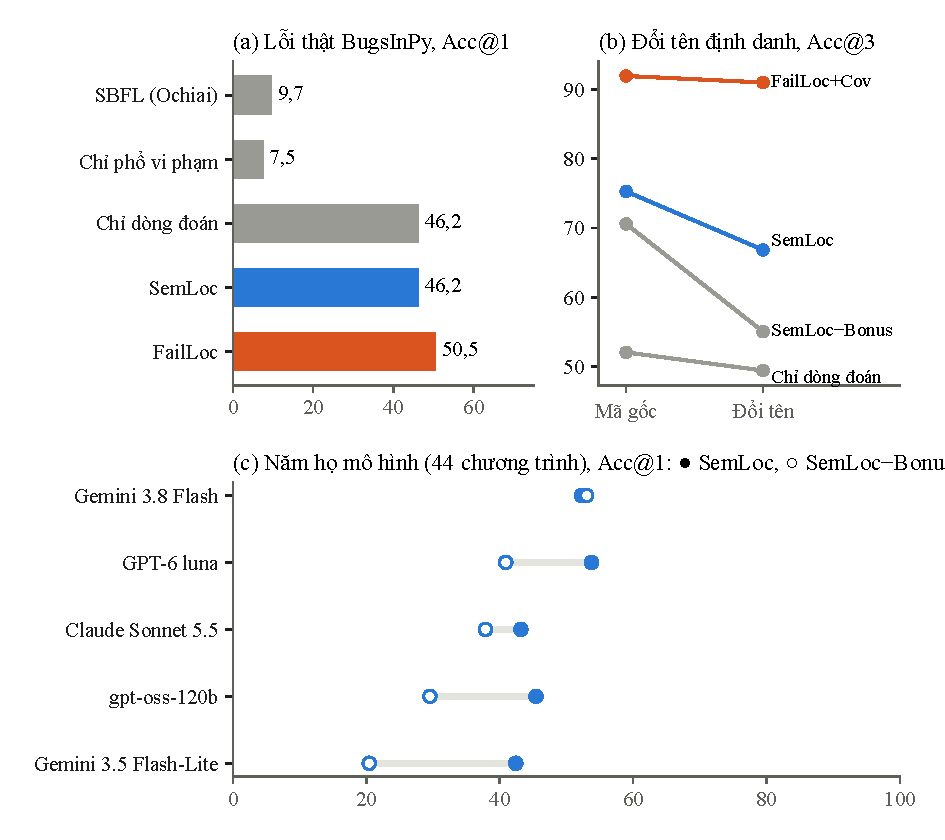
\includegraphics{../generated/vi/fig_rq3.pdf}
\caption{Độ bền: (a) lỗi thật BugsInPy, (b) trước và sau khi đổi tên định danh, (c) năm họ mô hình trên một tập con cố định của tập test}
\label{fig:rq3}
\end{figure}

\section{Phân tích thất bại và thảo luận}
\label{chap:that-bai}

Mục này hỏi: khi SemLoc (hoặc dòng LLM tự đoán) sai, nó sai thế nào và vì sao? Phân tích dùng ba lần chạy
Gemini 3.8 Flash trên tập test với nhãn đã chuẩn hóa; tín hiệu của mỗi chương trình lấy theo đa số ba lần.

\subsection{Sáu nhóm kết quả và năm mẫu nguyên nhân}
\label{sec:phan-nhom}

Mỗi chương trình được xếp vào đúng một nhóm, theo thứ tự ưu tiên: \texttt{gt\_suspect} (dòng lỗi chuẩn chưa kiểm chứng
được và mọi phương pháp trượt top-3), \texttt{guess\_right} (dòng LLM tự đoán là dòng lỗi chuẩn), \texttt{prior\_hurts}
(phổ xếp dòng lỗi hạng 1 nhưng điểm thưởng đẩy dòng đoán sai lên trên), \texttt{rescued\_by\_spectrum} (đoán sai nhưng
SemLoc vẫn có dòng lỗi trong top-3), \texttt{coverage\_only\_wins} (SemLoc trượt top-3, FailLoc+Cov trúng) và
\texttt{all\_miss}. Hình~\ref{fig:that-bai} cho số chương trình mỗi nhóm: trên \FailProgramsN{} chương trình, khoảng một
nửa được giải quyết bởi chính dòng tự đoán; bằng chứng thực thi chỉ ``cứu'' SemLoc ở \FailRescuedBySpectrumN{} chương trình.

\begin{figure}[H]
\centering
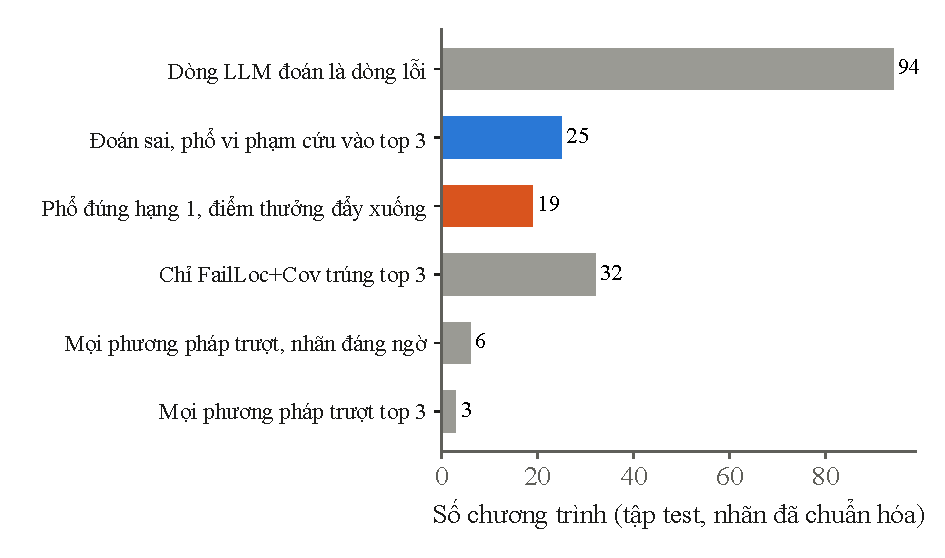
\includegraphics{../generated/vi/fig_failures.pdf}
\caption{Phân nhóm kết quả của SemLoc theo chương trình (tập test, nhãn đã chuẩn hóa, đa số ba lần chạy)}
\label{fig:that-bai}
\end{figure}

\label{sec:mo-ho}%
Dòng đoán lệch có hệ thống xuống dưới: trùng dòng lỗi chuẩn \OffLlmGuessZeroCount{} lần, lệch xuống một dòng
\OffLlmGuessOneCount{} lần nhưng lệch lên một dòng chỉ \OffLlmGuessMinusOneCount{} lần. Trong \FailWrongGuessN{} chương
trình đoán sai, \FailRelationHeaderBodyN{} ca có dòng đoán và dòng lỗi chuẩn là đầu một câu lệnh ghép và câu lệnh nó bảo
vệ. Chấp nhận cả hai dòng của cặp này thì Acc@1 của SemLoc tăng từ \TolSemlocAccOneExact\% lên
\TolSemlocAccOneGuardStrict\%--\TolSemlocAccOneGuardOrBody\%, của FailLoc+Cov từ \TolLlmCoverageAccOneExact\% lên
\TolLlmCoverageAccOneGuardStrict\%--\TolLlmCoverageAccOneGuardOrBody\%: quy ước gán nhãn ảnh hưởng tới Acc@1 nhiều hơn
mọi khác biệt giữa các phương pháp dùng LLM và đủ để đảo thứ tự giữa chúng (LLM-Direct từ đầu xuống cuối), dù FailLoc+Cov
vẫn hơn SemLoc. Đọc mười chín ca (tối đa bốn ca mỗi nhóm,
khác khuôn mẫu) cho năm mẫu nguyên nhân:
\begin{enumerate}
\item \textbf{Dòng điều kiện và câu lệnh được bảo vệ} (phổ biến nhất): nhãn ở \texttt{if}, LLM chỉ câu lệnh bên trong
  hoặc ngược lại; đúng về ngữ nghĩa nhưng lệch một dòng.
\item \textbf{Khối lỗi nhiều dòng}: xóa dòng nào cũng sửa được; nhãn nêu một dòng, LLM chỉ dòng kia (phần lớn \texttt{prior\_hurts}).
\item \textbf{Bộ phán định chấp nhận bản sửa bù trừ}: bản sửa làm mọi kiểm thử đạt ở một dòng không có lỗi. Bộ phán định
  chỉ xác nhận câu lệnh bằng bản thay thế và chỉ điền dòng trống hay chèn dòng khi không câu lệnh nào gần đó sửa được, nên
  không còn ghi đè bằng dòng chèn thêm; bản thay thế bù trừ thì vẫn lọt: vòng rà soát bác \ReviewCorrectedOverturnedN{}
  trong \GtCorrectedN{} lần bộ phán định dời nhãn.
\item \textbf{Nguyên nhân và triệu chứng trên cùng luồng dữ liệu}: nhãn ở nơi tính giá trị, LLM chỉ nơi dùng (hoặc ngược
  lại), hay lỗi là \emph{thiếu} một bước, không có ``dòng sai'' duy nhất.
\item \textbf{Dòng lỗi chuẩn đáng ngờ}: nhãn gán cho dòng khai báo hàm lồng hay cho dòng ngay trên lỗi rõ ràng.\end{enumerate}
Vì vậy không thể suy ra ``bỏ điểm thưởng thì tốt hơn'': các ca điểm thưởng ``gây hại'' gần như toàn là cặp đầu khối --
thân khối hoặc khối lỗi nhiều dòng. Điều còn thiếu là cách đánh giá chấp nhận các vị trí sửa tương đương.

\subsection{Thảo luận}
\label{sec:thao-luan}

\textbf{Kiểm thử đủ để gợi ý lỗi nhưng quá yếu để làm trọng tài.} Bằng chứng thực thi có ích ở top-3
(\FailRescuedBySpectrumN{} chương trình được phổ cứu, \FailCoverageOnlyWinsN{} chương trình SemLoc trượt nhưng FailLoc+Cov trúng), và
phần có ích là kiểm thử thất bại chứ không phải độ phủ (mục~\ref{sec:rq3}). Nhưng ba hiện tượng có chung một tiêu chí: bước vá thử của SemLoc
không đổi thứ hạng nào, bộ phán định dời \ReviewCorrectedOverturnedN{} nhãn tới dòng bị vòng rà soát bác, và FailLoc+Verify
không cải thiện bước đề xuất. Tiêu chí đó là \emph{một bản sửa nhỏ tại dòng này làm mọi kiểm thử đạt}. Với
khoảng mười kiểm thử mỗi chương trình, tiêu chí này thỏa ở \PavmechReviewedOtherLineFixable\% lần thử tại các dòng ứng
viên không có lỗi (tập dev, nhãn đã rà soát), thường bằng cách đổi một hằng số để bù cho phép tính sai ở chỗ khác, nhưng chỉ
\PavmechReviewedFaultLineFixable\% tại dòng lỗi thật (lỗi hai dòng hay lỗi thiếu mã không sửa được bằng một thay đổi nhỏ).
Đây là hiện tượng ``bản vá hợp lệ bề ngoài''~\cite{qi2015kali,smith2015cure}, nhìn từ phía định vị lỗi: bộ kiểm thử đủ
để \emph{gợi ý} lỗi ở đâu nhưng quá yếu để \emph{chứng minh} lỗi ở đâu.

\textbf{Bộ dữ liệu bão hòa.} Trên nhãn đã rà soát, FailLoc đạt Acc@3 \RqTwoReviewedAllLlmTestsAccThreeMean\%: hàm ngắn,
lỗi nhỏ, tên kiểm thử nói gần như thẳng ý định bị vi phạm; trên lỗi thật (mục~\ref{sec:rq4}) mọi phương pháp còn xa trần.
